\documentclass[12pt]{article}
\usepackage[utf8]{inputenc}
\usepackage{amsmath, amsthm, amssymb}
\usepackage[letterpaper, margin=1in]{geometry}
\usepackage{microtype}
\usepackage{enumitem}
\usepackage{biblatex}
\usepackage{mathtools}
\usepackage{amssymb}
\usepackage{float}
\usepackage{commath}
\usepackage{color}
\usepackage{wrapfig}

\addbibresource{main.bib}

\newtheorem{theorem}{Theorem}[section]
\newtheorem{corollary}{Corollary}[theorem]
\newtheorem{lemma}[theorem]{Lemma}
\newtheorem{alg}[theorem]{Algorithm}
\newtheorem{claim}[theorem]{Claim}

\theoremstyle{definition}
\newtheorem{definition}{Definition}[section]

% Commonly used symbols
\newcommand{\fiu}{f_{i}^{\mu}}
\newcommand{\nfiu}{\nabla \fiu}
\newcommand{\biu}{b_{i}^{\mu}}
\newcommand{\gie}{\gamma_{e}^{\mu}}
\newcommand{\giij}{\gamma_{ij}^{\mu}}
\newcommand{\vnott}{V \setminus t}
\newcommand{\din}{\delta^{in}}
\newcommand{\dout}{\delta^{out}}
\newcommand{\vpos}{V^{t}}
\newcommand{\vneg}{V^{s}}

\newcommand{\rewrite}[1]{\textcolor{red}{#1}}
\newcommand{\todo}[1]{\colorbox{yellow}{TODO: #1}}

\newcommand{\lpeq}[1] {
\begin{equation*}
\begin{aligned}
#1
\end{aligned}
\end{equation*}
}
\newcommand{\lpone}[3] {
& \underset{}{\text{#1}}
&& #2 \\
& \text{s.t.}
&& #3 
}
\newcommand{\lptwo}[4] {
\lpone{#1}{#2}{#3}\\
&&& #4
}
\newcommand{\lpthree}[5] {
\lptwo{#1}{#2}{#3}{#4}\\
&&& #5
}

\title{Strongly Polynomial Algorithms for Generalized Flow Maximization}
\author{Frank Cangialosi, Katie Lewis, David Palmer}
\date{}

\begin{document}
\maketitle
\section{Introduction}
	\subsection{Problem Definition} As in the traditional flow problem, given a graph $G = (V,E)$, the generalized maximum flow problem aims to maximize the total flow delivered to the sink node t $\in$ V. Unlike the original flow problem however, each edge contains a gain factor $\gamma_e$ $>$ 0, which scales the flow passing through that edge. Intuitively, this rescaling can be thought of in terms of real world examples such as exchange rates between currencies or physical transformations due to energy dissipation. The generalized maximum flow problem lacks several nice properties that are present in the traditional maximum flow problem, which makes it more challenging to solve. For example, the generalized problem is usually thought to be \rewrite{non-integral and, due to the scaling,} the total supply is not necessarily equal to the total demand. Additionally, the maximum flow-minimum cut theorem no longer applies since the flow along a path is not equal at every edge along that path.
    
    Until recently, the best known algorithms were all weakly polynomial. In 2013, \cite{Vegh2013} developed the first strongly polynomial algorithm (i.e. one that depends only on the number of nodes and edges in the graph, and is independent of the size of their values). In 2017, \cite{Olver2017} built on this work and developed an algorithm that is faster by a factor of almost $O(n^2)$, resulting in a running time that is as fast as the best weakly polynomial algorithms even for small parameter values. These algorithms take advantage of the structural similarities between the generalized maximum flow problem and the minimum cost flow problem by adapting techniques from well-known combinatorial min cost flow algorithms. 
    
	\subsection{Structure and Contributions of the Paper} In this paper, we aim to familiarize the reader with the recent algorithmic developments for the generalized flow maximization problem and provide intuition for the techniques used to achieve a strongly polynomial result. In Section 2, we more formally define the problem as a linear program and give an overview of the notation used in the rest of the paper. In Section 3, we develop the key techniques shared by both algorithms used to achieve a strongly polynomial bound for this problem. In Section 4, we describe Végh's original $O(n^3m^2)$ strongly polynomial algorithm developed in 2014 and present a more intuitive and detailed analysis than the original paper. In Section 5, we describe Olver and Végh's faster $O((m + n\ log\ n)mn\ log(n^2 / m))$ algorithm and highlight key aspects of the analysis that led way to the improved running time efficiency. Finally, in Section 6, we conclude with open questions and present a few ideas for future work. \todo{Update when we're done.}
    
\section{Preliminaries}

	\subsection{Network Notation}
    Let $G=(V,E)$ denote a directed graph with $n=\abs{V}$ and $m=\abs{E}$ and sink node $t \in V$. We define $\gamma \in \mathbb{R}_{>0}^E$ to be the vector of gains and $b \in \mathbb{R}^{V \setminus t}$ to be the vector of node demands. In this paper, we analyze networks with demands rather than capacities; however, this can easily be transformed into the capacitated (standard) representation \cite{Vegh2013}. We define $\delta^-(S)$ and $\delta^+(S)$ as the set of incoming and outgoing arcs of the subset S $\subseteq$ V. We denote the net flow as $\nabla$f$_i$ $\coloneqq$ $\sum_{e \in \Delta^-(i)}$ $\gamma_e$f$_e$ - $\sum_{e \in \Delta^+(i)}$ f$_e$. The residual graph is defined as G$_f$(V,E$_f$), where the set of edges E$_f$ = E $\cup$ $\{$ ji: ij $\in$ E, f$_{ij}$ $>$ 0 $\}$ contains the original edges and reverse arcs. We define $\gamma_{ji}$ $\coloneqq$ $\frac{1}{\gamma_{ij}}$ and f$_{ji}$ $\coloneqq$ -$\gamma_{ij}f_{ij}$. If a cycle C in the residual graph has $\prod_{e \in C}$ $\gamma_e$ $>$ 1, we call the cycle a flow generating cycle.
    
    \todo{Add more notation? eg define excess, surplus?}, \todo{Add example diagram}
    
    \subsection{Linear Program Formulation}
    \label{sec:lp}
    
    The generalized flow maximization problem with demands can be formulated as the following LP:
    
        \begin{align*}\tag{P}
        \text{max} \quad
        \nabla f_t& \\
        \text{s.t.} \quad
        \nabla f_i &\geq b_i \quad \forall i \in V \setminus t \\
        f &\geq 0
        \end{align*}        

\noindent The corresponding dual:
 
        \begin{align*}\tag{D}
        \text{max} \quad
        \mu_t &\sum_{j \in V \setminus t} \frac{b_j}{\mu_j}  \\
        \text{s.t.} \quad
        \mu_j &\geq \gamma_{ij}\mu_i \quad \forall ij \in E \\
        \mu_t &\in \mathbb{R}_{++} \\
        \mu_i &\in \mathbb{R}_{++} \cup \infty \quad \forall i \in V \setminus t
        \end{align*}  
        
A feasible solution, $\mu$, to the dual is known as feasible labeling. We can interpret a label $\mu_i$ as a changing in the base unit of measurement  at node i (for example measuring in pennies instead of dollars). We can transform the dual problem to be comparable to the original problem by relabeling the flow, net flow, gains, and demands as follows:

\begin{align*}
f_{ij}^\mu \coloneqq \frac{f_{ij}}{\mu_i} \quad
\nabla f_i^\mu \coloneqq \frac{\nabla f_i }{\mu_i} \quad
\gamma_{ij}^\mu \coloneqq \gamma_{ij} \frac{\mu_i}{\mu_j} \quad
b_i^\mu \coloneqq \frac{b_i}{\mu_i} \quad
\end{align*}

An arc in the relabeled graph is known as tight with respect to $\mu$ if $\gamma_e^\mu$=1. The excess and deficit of a node i in the relabeled graph is defined as:


\begin{align*}
Ex(f,\mu) \coloneqq \sum_{i \in V - t} max\{ \nabla	f_i^\mu - b_i^\mu, 2 \} \\
Def(f,\mu) \coloneqq \sum_{i \in V -t} max \{ b_i^\mu - \nabla f_i^\mu, 0\}
\end{align*}

\todo{Explanation of the dual variables and constraints, and intuition behind them}
  
\section{Motivating Ideas and Techniques}
	\subsection{Solving Dual}
    	* Talk about idea of solving dual 
        	* Key insight about this algorithm is that they maintain f$^{\mu}$ (without any extra work apparently) to be integral
            * Allows normal flow algorithms 
            * Is maintaining solution that is "close enough to feasible primal" with complementary slackness unique to this algorithm?
            * Draw parallels between min cost flow and generalized max flow (give more clear and intuitive explanation than the Truemper paper)
            
	The algorithm solves the primal generalized flow problem by first solving the dual problem.
    A solution to the dual problem specifies, by complementary slackness, the arcs on which an optimal
    primal solution may send flow. Moreover, applying the dual labels regularizes the problem, reducing
    it to an ordinary circulation problem. Starting from dual labels $\mu$, $f^{\mu}$ must satisfy
    \[ \sum_{j \in \delta^-(i)} \gamma^\mu_{ij} f^\mu_{ij} - \sum_{j \in \delta^+(i)} f^\mu_{ji}
     = \nabla f^{\mu} \geq b^{\mu}, \]
    but $\gamma^{\mu}_{ij} = 1$ whenever $f_{ij} \neq 0$. So the dual solution reduces the primal problem
    to an ordinary maximum flow problem with demand constraint.
     
    This suggests an algorithm that 
    
    \subsection{Contracting Arcs}
    

\section{The Initial Strongly Polynomial Algorithm}
\section{A Faster Strongly Polynomial Algorithm} The improved strongly polynomial algorithm developed by Olver and Végh \cite{Olver2017} introduces several new conceptual ideas that combine the techniques and insight from Section 3. In this section, we will give an overview and analysis of their algorithm. We will also provide a more clear distinction between the previous techniques used and the new insights provided by this algorithm (and why they matter). A highlight of the difficulties in previous algorithms and the subsequent solutions from this algorithm are summarized in Table~\ref{tab:improvements}.

\begin{table}[H]
\begin{center}
    \begin{tabular}{ | p{7cm} | p{7cm} |}
    \hline
    Challenges in Previous Algorithms  & Solutions from New Algorithm \\ \hline
    Non-integral flow values & Only store relabeled flow $f^{\mu}$ which stays integral throughout the algorithm until the last step of computing optimum \\ \hline
    Initial cycle-canceling algorithm to eliminate flow generating cycles & Two phase method (similar to simplex) where feasible solution found in first phase is used to start the second phase; this solution is faster than the cycle-canceling subroutine \\ \hline
    Complex methods for maintaining feasible flow & Relax flow feasibility (node demands do not have to be met) and use complementary slackness properties to keep feasible primal solution "within reach" \\ \hline
    No guarantee of abundant arc appearing in strongly polynomial number of steps \cite{Radzik2004} &  Continuous scaling\\ \hline
    Complicated multiplicative potential analysis \cite{Vegh2013} & Additive potential analysis \\
    \hline
    \end{tabular}
\end{center}
\caption{Key Improvements of New Algorithm}
\label{tab:improvements}
\end{table}
    \subsection{Additional Notation and Concepts}
At each iteration of the algorithm we ensure that we have a \textbf{fitting pair} of primal-dual solutions $(f,u)$ such that $\mu$ is a feasible dual solution, and $\gamma_e^{\mu}$ is 1 (tight) for all edges with flow on them $(f_e > 0)$. \todo{Provide small diagram with numbers and show calculation of $\mu$ given $f$ or vice-versa.} Notice that this relaxed definition does not require that $f$ is feasible (i.e. we allow the net flow $\nabla f $ to be less than its demand $b$). Rather than going through extra work of maintaining a feasible $f$ at each step, a key contribution is simply ensuring that a feasible $f$ \textit{exists} for the $\mu$ in our fitting pair. We denote such a $\mu$ as \textbf{safe}. Further, since all arcs in $f$ are tight, this definition ensures that the scaled $f$, $f^{\mu}$, is a ``regular'' flow and thus one can use any traditional algorithm to manipulate it. As a result, given a fitting pair where the dual solution is optimal, one can find an optimal primal solution by solving a feasible circulation problem \todo{why the circulation problem?}. 

    \subsection{Finding a feasible flow}
Drawing inspiration from the Simplex algorithm, the first step in this algorithm is finding a trivial feasible solution $(\bar{f}, \bar{\mu})$, which clearly also satisfies the definition of a fitting pair necessary for the algorithm. In order to find this initial solution, rather than using Radzik's cycle-cancelling subroutine as in prior work, the authors develop a new method based on negative cycle detection, which can be run in $O(nm)$ time. \todo{references} 
    
    \subsection{Scaling and Rounding} 
    Since the second phase of the algorithm relies on the relabeled flow, f$^\mu$, being integral, we must first round the initial feasible flow (which does not have an integrality constraint) and then maintain its integrality throughout the second phase until finding the final optimum. Using the integrality properties of maximum flow, we can run a feasible circulation problem on the relabeled graph to find an integral max flow. We do this by taking the initial fitting pair (f,$\mu$) and corresponding feasible relabeled flow f$^\mu$ and setting a lower bound of $\lfloor$$\nabla$f$_i^\mu$ $\rfloor$ and an upper bound of $\lceil$$\nabla$f$_i^\mu$$\rceil$. The corresponding integral relabeled max flow on each edge e$_{ij}$ can be turned into an integral flow by multiplying by $\mu_i$. Throughout the second phase, the value of f$_{ij}^\mu$ remains unchanged because if f$_{ij}$ is scaled, the algorithm scales $\mu_i$ by the same amount; therefore, f$_{ij}^\mu$ remains integral after the initial rounding.
    
    In addition to rounding the initial feasible flow, the initial labels, $\mu$, are scaled at the beginning of phase 2. Before rounding, we set a scaling factor $\Delta$ equal to max$_{i \in V -t}$ $\nabla$f$_i^\mu$ - b$_i^\mu$, which is the maximum excess at a node in the initial feasible solution. We multiply $\mu$ by $\Delta$, which is reduces f$^\mu$ by a factor of $\Delta$. This scaling is useful because it bounds $\nabla$f$_i^\mu$, which is used to bound the total excess in the amortized analysis (explained in Section 5.8). The resulting bound is $b_i^\mu - 1 \leq \nabla f_i^\mu \leq b_i^\mu + 2 \quad \forall i \in V-t $; the derivation leading to this result is not explicitly explained in the original paper \cite{Olver2017}, but we provide a clearer explanation. Initially, $\nabla f_i^\mu \geq b_i^\mu$ because it must be feasible. After rounding, $\nabla f_i^\mu \geq b_i^\mu - 1$ because $\nabla f_i^\mu$ decreases by at most 1. This gives the lower bound of the result. The upper bound comes from the scaling and the definition of Ex(f,$\mu$) in Section~\ref{sec:lp}. Since we scale $\nabla f_i^\mu$ down by the maximum excess in the initial solution, the maximum in Ex(f,$\mu$) will never be $>$2. This gives the upper bound $\nabla f_i^\mu \leq b_i^\mu + 2$ on $\nabla f_i^\mu$. 

\subsection{Plentiful Nodes}

\subsubsection{Movation}

Recall that the primary method of progress in this algorithm involves
identifying contractible arcs (\todo{define}) and then contracting them until a dual optimal
solution is found. Prior work called such arcs ``abundant'' and used scaling to
find them directly. A key novelty in this algorithm is the concept of finding
them indirectly via a ``plentiful'' node. 
\begin{definition}
We say that a node $i$ is \textbf{plentiful} with respect
to our current primal-dual solution pair $(f,u)$ if its scaled absolute
demand $|b_i^{\mu}|$ is large relative to the size of the graph, specifically:
$|b_i^{\mu}| \ge 3n(d_i + 1)$.
\end{definition}

It is important to notice that, just as with the definition of an abundant  arc,
this definition depends only on the size of the graph, which is a key property
that will keep our algorithm strongly polynomial because we will be iteratively
re-scaling the node demands until one of them satisfies this property.

\begin{theorem} Assume $\mu$ from the fitting pair $(f,\mu)$ is safe.
Then the existence of a plentiful node $i$ ensures
that there exists a contractible arc $e$ incident to $i$.
\end{theorem}
\begin{proof}
\todo{Prove theorem 3.1 more succinctly and clearly}. General idea: 
\end{proof}
\todo{Example of why this fails if $\mu$ is not safe. See appendix to 2017.}

\subsubsection{Subroutine: Producing Plentiful Nodes}
\label{sec:sub-ppn}

For an input fitting pair $(f,u)$ without a plentiful node, the algorithm
repeatedly alternates between two steps which adjust the primal and dual
solutions until at least one node becomes plentiful.

First, the primal solution is improved by augmenting as much flow as possible,
one unit at a time, along tight arcs in the residual graph 
from nodes with excess to either nodes with deficit, or the sink.
It only augments along tight arcs \rewrite{because}. Formally, if we let
$D$ (``destinations'') be the union of the sink $t$ and all nodes with 
deficit ($\nabla f_i^{\mu} < b_i^{\mu}$), and let $S$ (``sources'') be
the set of all nodes that both have excess ($\nabla f_i^{\mu} \ge \lceil b_i^{\mu} \rceil$)
and have a tight path in the residual graph to a node in $D$, then the algorithm
continues augmenting until $S$ is empty.

Once it is not possible to augment any more flow, the second step scales down
the labels and flow for all nodes and edges in $S$ by the same factor $\alpha$,
which is chosen to be the largest value that \rewrite{does not violate} any of the dual
constraints~(\ref{eq:dual}) or produces a plentiful node. 
Although it is not necessary in practice, for clarify of explanation, one can think of choosing the scaling factor $\alpha$ as solving
the following LP:
\lpeq{\lpthree{max}
{\alpha}
{\gamma_{ij}^{\mu} \le 1\ \forall\ i,j \in \din(S)}
{\nfiu - \biu \le 1}
{\nexists\ \text{plentiful}\ i \in \vpos}
}
\begin{figure}[b!]
\centering
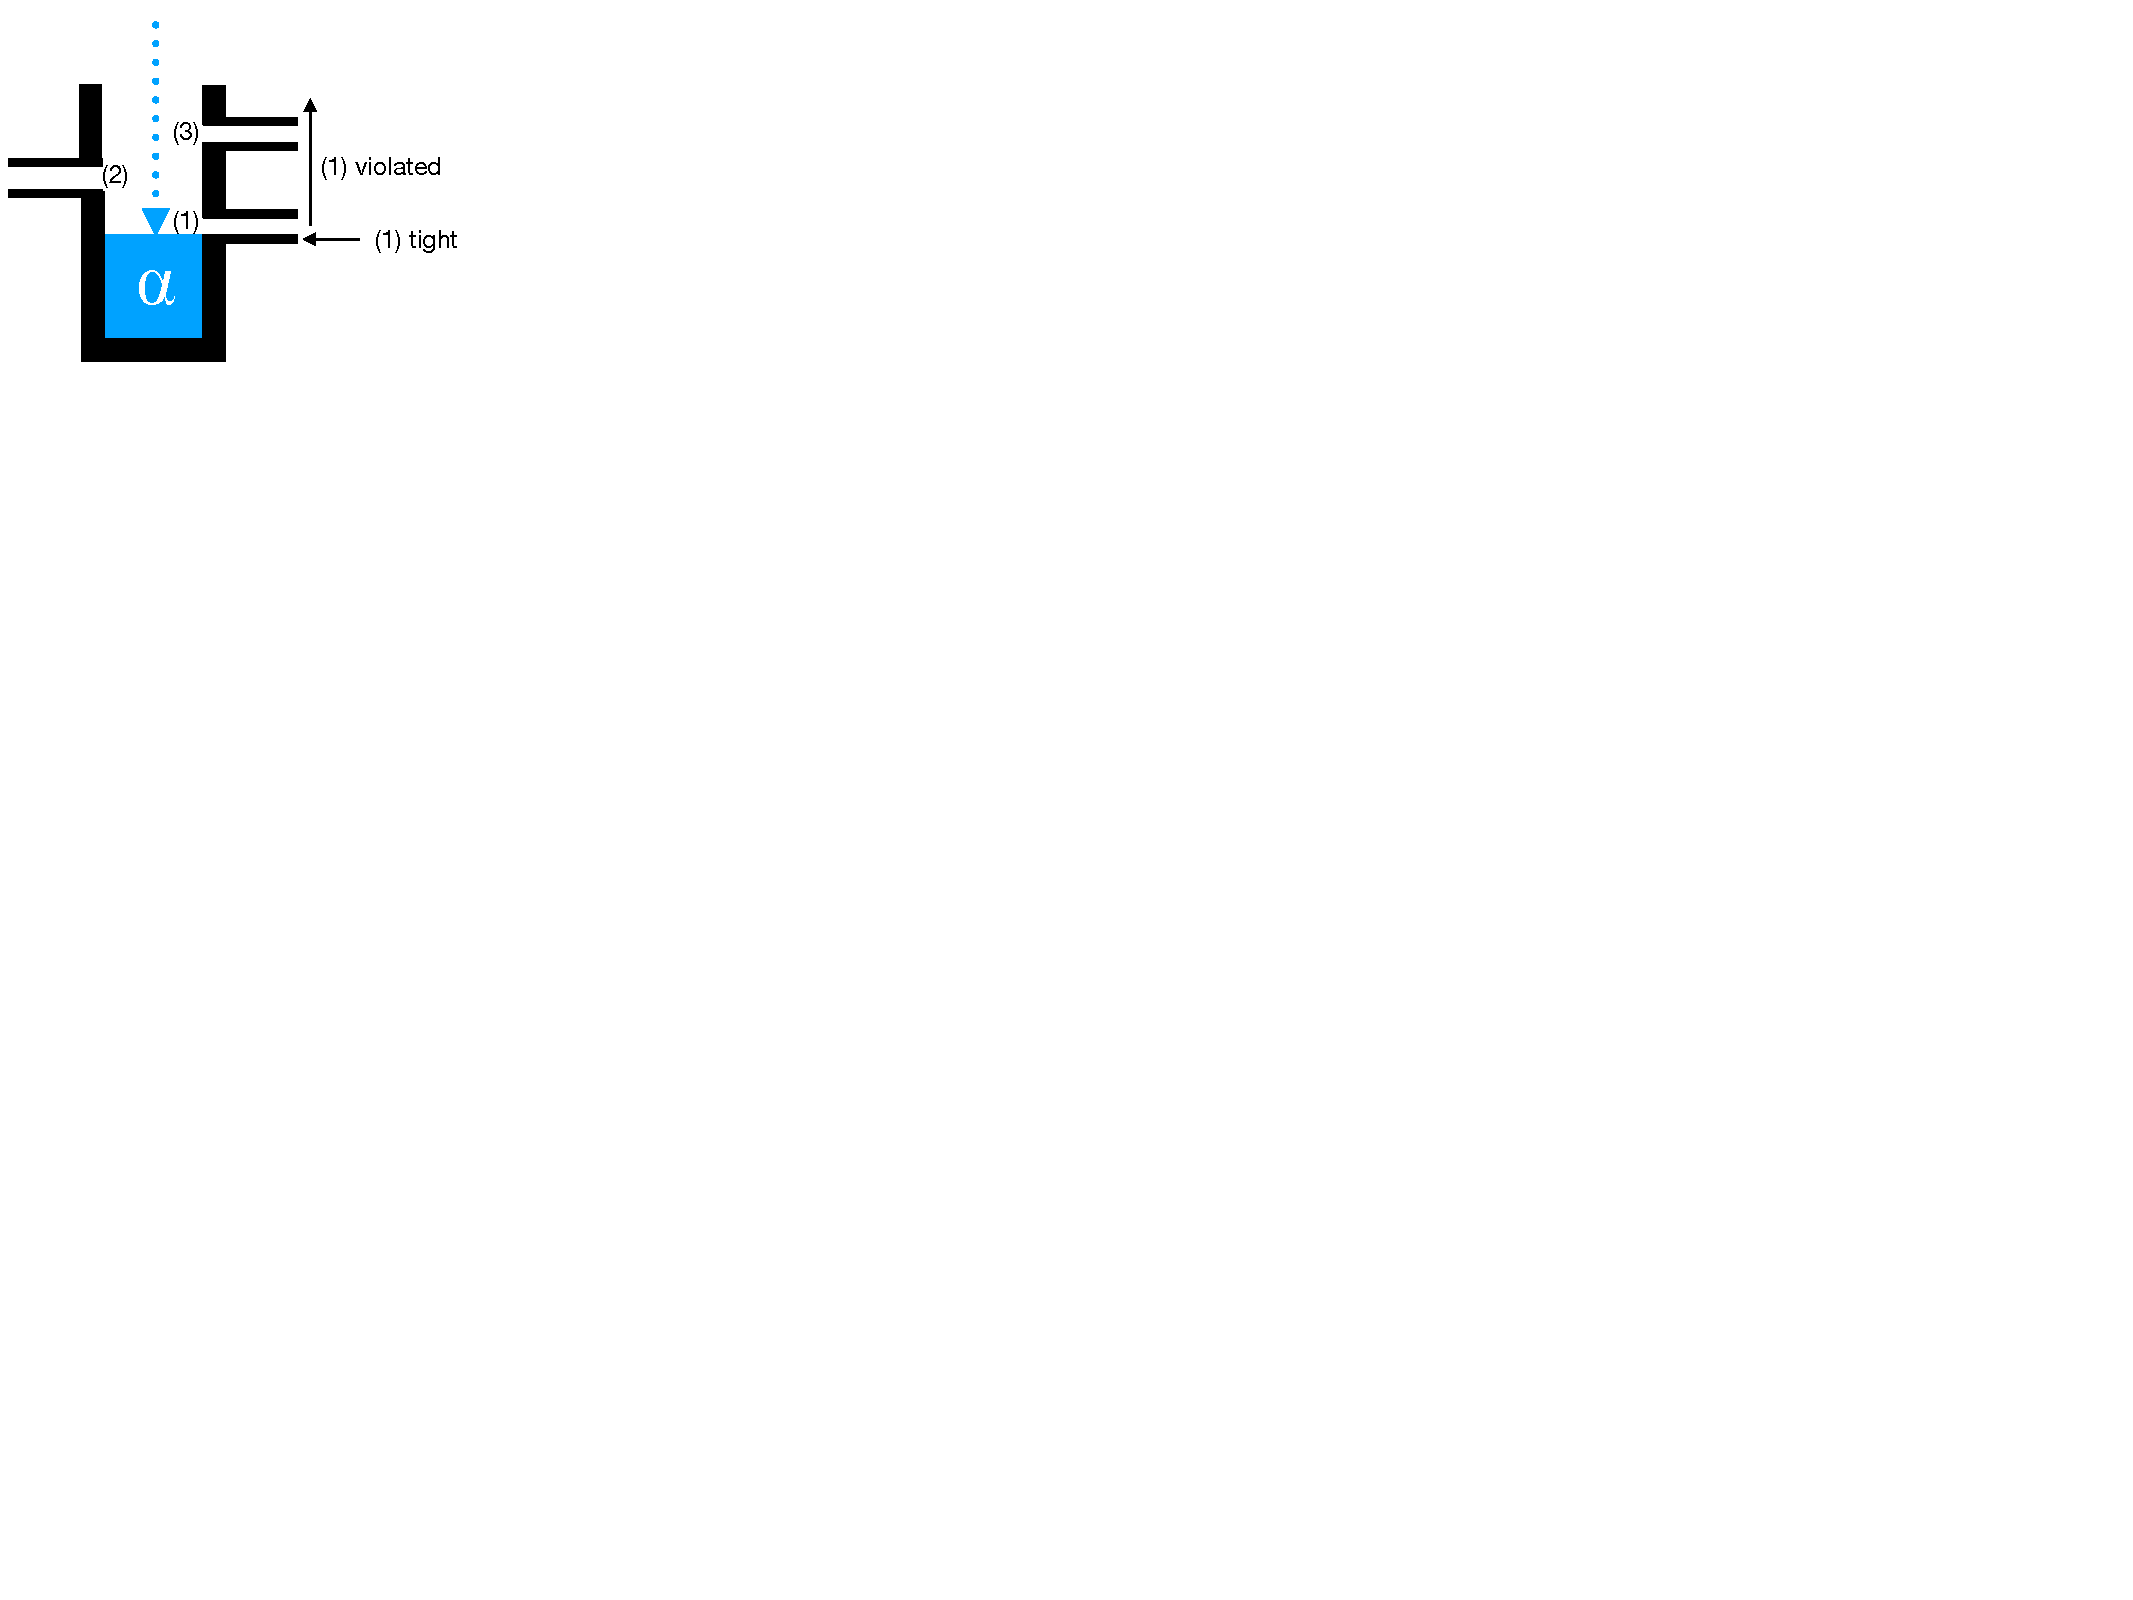
\includegraphics[width=0.35\textwidth]{figs/water.pdf}
\caption{
\label{fig:alpha}
Informal analogy for the maximization of scaling parameter $\alpha$.
Each pipe represents a constraint. $\alpha$ can only be increased until
one of them becomes tight as increasing it further would leak into
the lowest pipe and violate that constraint.
At each step, the order of which constraint becomes tight first may be different.
}
\end{figure}
Intuitively, as illustrated in Figure~\ref{fig:alpha}, this is akin to filling
a basin with water as much as possible without any of the water leaking into one
of three pipes, where each pipe represents a constraint and its height in the basin
represents the value of $\alpha$ at which point it becomes tight.

Thus, $\alpha$ is chosen such that one of the following constraints becomes
tight, or, in other words, one of the following becomes true corresponding to
each constraint, respectively:
\begin{enumerate}[itemsep=-1mm]
	\item An edge entering $S$ becomes tight, and thus a new node is added to $S$
	\item A node in $S$ has excess $>1$, which allows us to augment flow from it
	\item A pseudosink node becomes plentiful
\end{enumerate}

If (3) is true, we're done. If (1) or (2) are true, it ensures that we will now
be able to make progress in the next iteration of the first step. Similarly, the
augmentations in the first step

Although it is conceptually easier to imagine increasing $\alpha$ continuously
until one of these constraints becomes tight, in practice, it is possible to
calculate $\alpha$ arithmetically in $O(n)$ by picking a value for each node
that would satisfy one of the tightness conditions and then choosing the minimum
such value so that only one of the constraints become tight and none are
violated.
The details of calculating the value are not particularly insightful, but the
fact that it can be done is important for the running time analysis.

We now make some important claims about the variables as the algorithm
progresses that allow us to prove its correctness: i.e. that it terminates,
producing a plentiful node.
We prove further that it terminates in strongly polynomial time and derive an upper bound 
in the following section.

\begin{claim}
$f^{\mu}$ remains unchanged throughout the subroutine.
\label{lem:fsame}
\end{claim} 
\begin{proof}
By definition, only arcs $(i,j) \in S$ are 
\end{proof}
\begin{corollary}
$f^{\mu}$ is always integral.
\end{corollary}
\begin{proof}
The augmentation step clearly maintains integrality of $f^{\mu}$ because we
always augment by 1 unit at a time. The only other part of the algorithm that
modifies the primal solution is the relabeling of $f_e$, and by the previous
claim (\ref{lem:fsame}), this never changes the value of $f^{\mu}$.
\end{proof}
\begin{claim}
	For all nodes with non-zero demand in $S$, scaling $\mu$ in the second step
	strictly increases $|\biu|$. For all other nodes, $|\biu|$ remains unchanged.
\end{claim}
\begin{proof}
	First, trivially, scaling a node with zero demand cannot change its value
	($0\cdot\mu=0$), and the algorithm only updates $\mu_i$ for $i \in S$. Recall
	that $\biu$ is defined as $\frac{b_i}{\mu_i}$, and thus, if $\mu_i\leftarrow \mu_i / \alpha$,
	then $\biu \leftarrow \frac{b_i}{\mu_i / \alpha} = \alpha\frac{b_i}{\mu_i} = \alpha \biu$. 
	Now it suffices to prove that $\alpha > 1$ always holds when any of the three
	constraints become tight.
	
	By construction, before rescaling, $S$ has no tight
	incoming arcs. Recall $\giij = \gamma_i\frac{u_i}{u_j}$. In order for an
	incoming arc $i \notin S, j\in S$ to become tight (1), we must have $\giij=1$:
	since we only scale values in $S$, $\alpha$ must be ${1}/{\giij}$, which is
	always greater than $1$ because $\giij < 1$ (by the feasibility of the dual).

	From the terminating condition of the augmentation step (the lack of any nodes
	in $S$ having excess), we know $Ex(f) = \nfiu - \biu < 1$. Since, by
	Lemma~\ref{lem:fsame}, $\nfiu$ is unchanged and only nodes in $\vneg$ (i.e. $b_i<0$)
	can have excess, the only way for to make $Ex(f) \ge 1$ is if $\biu$ becomes
	more negative, which only happens if $\alpha > 1$. 
	
	Finally, we start out with the assumption that there are no plentiful nodes.
	In order for a node to become plentiful (3), its demand $\biu$ must increase,
	which is only possible if $\alpha > 1$.
\end{proof}

In summary, we have shown that the primal and dual steps always allow room for the other to make progress, and collectively each iteration of the two steps strictly increases $|\biu|$ towards
the definition of a plentiful node. Thus, the subroutine will eventually produce one. We have also shown that the updates it makes to $f$ and $\mu$ do not violate any of the previous conditions stated for being able to ultimately derive a primal optimal solution once our fitting pair finds the dual optimal. 

\subsubsection{Running Time Analysis}

We now leverage potential analysis to derive an upper bound on the amount of work required for the subroutine introduced in Section~\ref{sec:sub-ppn} to terminate, showing that it is strongly polynomial, and confirming the analysis found in the paper. 

\todo{Proof}

\subsection{Contraction}

Once we have produced a plentiful node, finding a contractible arc is straightforward. 

The purpose of contraction is that it reduces the size of the graph by one node,
which puts a strongly polynomial bound of $n$ on the number of contraction
operations. 
\subsection{Expand to Original}
\subsection{Compute Primal}
\subsection{Amortized Analysis}





\section{Discussion and Future Work}

\subsection{Non-triviality of a strongly polynomial algorithm}

\todo{Explain} why applying ideas from strongly polynomial algorithms for
min-cost flow was not straightforward. 

\nocite{*}
\printbibliography
\end{document}
 
